\documentclass[a4paper,11pt]{article}
\usepackage[T1]{fontenc}
\usepackage[utf8]{inputenc}
\usepackage{lmodern}
\usepackage[french]{babel}
\usepackage{graphicx}
\usepackage{cite}
\usepackage{hyperref}

\title{%
  Rapport d'avancement thèse ACSEL \\
  \large Comité de Suivi Individuel 09/2018 \\ % Subtitle
  \large \textit{Sous la direction de David Defour, MCF HDR 27e et Bijan Mohammadi, Pr, 26e}}
\author{Christophe Pont}

\graphicspath{{illustrations/}}

\begin{document}

\maketitle
\tableofcontents

%\begin{abstract}
%\end{abstract}

%%% PRESENTATION
\section{Présentation}

% PRESENTATION PERSONNELLE
\subsection{Présentation personnelle}
Après l’obtention d’un Bac S spé maths (mention bien) à Toulouse, j’ai intégré un DUT Informatique, que j'ai obtenu avec la mention Bien. Mon cursus s’est prolongé à Polytech Montpellier, où j’y ai obtenu mon diplôme d’ingénieur en Informatique et Gestion (mention Bien). Durant cette formation, j’ai pu réaliser un stage anglophone dans un laboratoire de bioinformatique à l’université d’Ottawa, au Canada. Ce premier contact avec la recherche m’a incité à démarrer un doctorat, en octobre 2017, après deux ans en tant qu’ingénieur logiciel dans une grande entreprise de service informatique (SSII). L’idée était d’harmoniser mon orientation avec mon attrait pour la science, en particulier l’informatique et les mathématiques. C’est pourquoi je me suis dirigé vers le laboratoire LAMPS, et ai démarré mon doctorat sous la direction de David Defour, HDR, 27e afin de démarrer une thèse mêlant ma compétence informatique avec mon attrait pour les mathématiques : le tout, dans un contexte écologique qui me tient à cœur. J’aspire à continuer ma carrière dans la recherche, qui sait peut-être en tant que maître de conférence.

% PRESENTATION THESE
\subsection{Contexte}
Le contexte dans lequel se place mon sujet de thèse est double.
D’un côté, on s’intéresse à l’\textbf{arithmétique flottante}. Les nombres flottants sont une discrétisation des nombres réels. 
\begin{figure}[b]
  \begin{center}
    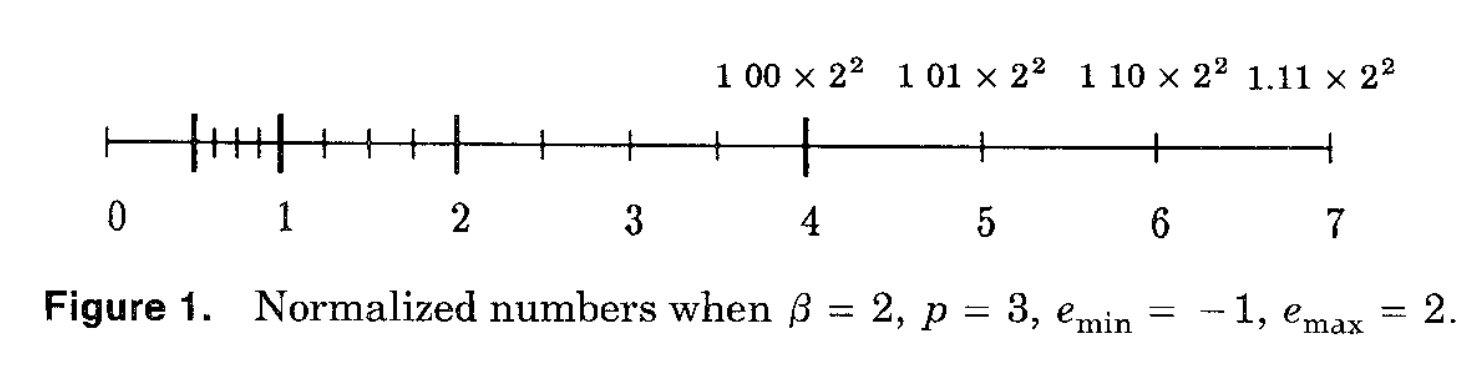
\includegraphics[width=12cm]{Floating_point_numbers_discretization}
    \caption{Exemple de discretisation des nombres réels en nombres flottants. Source : Goldberg, D. (1991). What every computer scientist should know about floating-point arithmetic. ACM Computing Surveys (CSUR), 23(1), 5-48.\cite{goldberg1991every}}
    \label{discretization}
  \end{center}
\end{figure}
Prenons l'exemple d'une discrétisation flottante des nombre réels (Figure ~\ref{discretization}) selon les paramètres suivants : $\beta=2, p=3, e_{min}=-1,e_{max}=2$, avec $\beta$ la base, $p$ la précision, $e_{min}$ l'exposant minimal, $e_{max}$ l'exposant maximal.
Sur l'exemple, on voit bien que $1,25$ est représentable ($1.01*2^{0}$), de même que $3$ ($1.10*2^{1}$). Bien que la somme de ces deux réels donne $3,25$, la somme flottante de ces deux nombres flottants donne elle $3$ (après arrondi), car $3,25$ n'est pas représentable exactement dans ces conditions.
Le Standard IEEE 754\cite{zuras2008ieee} définit 3 entiers $(s,e,m)$ pour représenter nombres flottants. Il fournit aussi des \textbf{formats}, qui définissent la façon dont chaque nombre flottant est \textbf{encodé}. On peut citer le format simple précision, le format double précision etc. \\
Malgré la définition d'un standard, l'arithmétique flottante est soumise à de multiples erreurs. On pense notamment aux \textbf{erreurs d'arrondi}, comme dans le cas cité ci-dessus, où $3,25$ a dû être arrondi à $3$, entraînant la \textit{perte} de $0,25$. Mais on peut aussi citer les \textbf{erreurs de cancellation}, qui surviennent lorsque l'on soustrait deux grandes valeurs très proches l'une de l'autre, révélant la perte de nombre significatifs lors de précédents calculs. \\ % TODO exemple.
Hors, lorsque l’on simule un modèle qui comprend de nombreux calculs (super calculateurs, vastes simulations à exécution longue), les différentes erreurs s’accumulent, se combinent, et finalement affectent le résultat.

Le deuxième volet de ma thèse porte sur ce domaine, celui de la \textbf{recherche d'erreurs numériques dans les programmes}.
Le cas d’étude de ma thèse porte sur les modèles et simulations de \textbf{Gladys}\footnote{\url{http://www.gladys-littoral.org}}.
Gladys est un réseau international de littoralistes en méditerranée, regroupant de nombreux chercheurs dans le domaine du littoral.
Ils ont établi de nombreux modèles pour décrire les phénomènes afférents à leur activité, notamment le phénomène \textbf{d’évolution du trait de côte}.
L’implémentation informatique de ce modèle sera le sujet d’étude de ma thèse (un code volumineux en C et Fortran). Il prend des données en entrée et réalise sa simulation. C'est ici que viendra se placer mon travail. L’idée sera de \textbf{compiler} le programme, et d’en produire une analyse visant à suivre et quantifier les erreurs liées à l’arithmétique flottante.

%modèle sur lequel a travaillé Bijan  [ accrétion, érosion ]
%les résultats subissent différents types d’erreurs [EDP, on dérive en fonction du temps, les erreurs peuvent s’accumuler/se combiner]
%objectif : quantifier l’erreur informatique, numérique

\subsection{État de l’art}

On peut distinguer deux catégories d'initiatives existantes dans le domaine : les démarches visant à “limiter” l’effet des erreurs (on peut citer les sommations compensées, Salsa...), et celles visant à quantifier et mesurer les erreurs.
Ma thèse fait écho à cette deuxième approche.
Je vais me baser sur une riche littérature existante.
De nombreux outils existent pour réaliser cette analyse, chacun ayant différentes entrées (programme, modèles, binaires…), et différentes contraintes.
On s’intéresse ici à deux approches probabilistes particulières : la méthode CESTAC, et l’arithmétique de Monte Carlo.
méthode CESTAC, qui va utiliser un grand nombre de tirages pour approximer efficacement le nombre de bits significatifs du résultat
DSA : basée sur CESTAC, redéfinit les opérateurs relationnels pour effectuer chaque opération N fois, en changeant aléatoirement le mode d’arrondi [ (nombres stochastiques, zéro stochastique)] 
Enfin, CADNA implémente DSA pour N=3, où les deux premiers modes d’arrondis sont choisis aléatoirement, et où le troisième est différent du second.
MCA, analyse de sensibilité
Verificarlo implémente MCA
FPANR, format proposé par David Defour, qui comme on va le voir encode astucieusement la précision dans la mantisse

MCA et DSA : deux méthodes probabilistes vérifier précision arithmétique
(Verificarlo prétend que les hypothèses de CESTAC ne tiennent pas : “je n’ai pas le recul pour m’exprimer sur le sujet”)

CESTAC : Controle et Estimation Stochastique des Arrondis de Calculs
DSA : Discrete Stochastic Arithmetic
CADNA : Control of Accuracy and Debugging for Numerical Application
SAM : Stochastic Arithmetic in Multiprecision
MCA : Monte Carlo Arithmetic
FP-ANR : Floating-Point Adaptive Noise Reduction

Analyse statique

\section{Travail réalisé}

\subsection{ arrondi randomisé }
inspiré de MCA
exemple RNDN arrondi toujours 0,49
résout potentiellement des problèmes d’accumulation d’erreurs d’arrondi

Entraîner des réseaux de neurones avec des formats restreint (en fixed-point), à faible précision, et observer la sensibilité de l’apprentissage au mode d’arrondi.
Quand ils diminuent trop la précision, on observe un phénomène de divergence. Pour compenser, ils introduisent un arrondi randomisé.
Ils observent dans ce cas que la différence peut aller d’une divergence du gradient à une convergence!
L’idée est donc de tester cet arrondi randomisé dans d’autres cas, et finalement reproduire leurs résultats.
Une piste intéressante pour expliquer cette convergence est que l’introduction de bruit s’avère positive dans l’apprentissage de CNN : on l’ajoute donc volontairement lors de l’entraînement. De la même façon, il serait intéressant de voir dans quelle mesure le bruit induit par l’arrondi stochastique pourrait avoir un impact sur l’apprentissage.


On a voulu tester l’arrondi randomisé sur des procédés connus pour être numériquement instables.
Applications : 
Gradient conjugué, procédé itératif, résout des systèmes d’équations linéaires.
Lorenz Procédé sensible à la précision dans les calculs flottants, donc potentiellement au mode d’arrondi utilisé.
“procédé itératif (llorenz), impact sur l’accumulation d’erreur ?”

l’implémentation a été assez complexe, puisqu’il fallait utiliser un mode d’arrondi codé “à la main” dans chaque opération

on exécute tout ça de multiples fois (1000 fois environ les premières fois si je ne m’abuse (évidemment le temps d’exécution s’en fait sentir))
Lorenz first

\subsubsection{lorenz}
On se compare à un run “optimal”, réalisé avec une forte précision, et on compare les valeurs intermédiaires à ce résultat.
Concernant les axes, on a deux échelles log, une pour le temps, les itérations, l’autre pour la distance à l’optimal (plus c’est haut, plus on s’éloigne).

On observe assez clairement l’accumulation d’erreur, car plus on avance plus on perd en précision 
CADNA semble fournir des résultats équivalents à ceux du mode d’arrondi standard, dans l’ensemble plus précis que l’arrondi randomisé

\subsubsection{gradient}
Gradient conjugué, pas grand chose à dire : malheureusement j’ai perdu les analyses le concernant en même temps que la défaillance de mon disque dur
on voit pas grand chose mais on voit que l’arrondi au plus près est légèrement meilleur que le randomisé.
Les métriques plus intéressantes qui sont venues après comparaient les deux modes d’arrondi en fonction du nombre d’itération, et non plus seulement de la précision des mantisses utilisées

[ l’objectif était de se lancer dans les réseaux de neurones, j’ai décidé de me lancer dans l’analyse des erreurs ]
Avant de me lancer dans l’extension aux réseaux de neurones, j’ai décidé de réaliser l’implémentation de FPANR en juin dernier.

\subsection{ FPANR }
L’idée est de proposer un encodage particulier d’un nombre flottant.
On a vu qu’au cours des calculs, un nombre flottant peut être amené à accumuler du bruit. Une partie de sa mantisse est alors non signifiante.
FPANR propose un mécanisme astucieux permettant de marquer la partie signifiante. (voir dessins) représentation de l’incertitude
On va encoder dans la mantisse l’incertitude : ce “coût” sera un motif non significatif à la fin du nombre flottant : qui, de toute façon, remplace des bits n’ayant pas de “sens”


s’inspire de Significance arithmetic
Encodage de l’information concernant  le nombre de bits significatifs directement dans la mantisse du nombre flottant, à l’aide d’un pattern
pas de surcoût mémoire : l’information est encodée directement dans la mantisse. Pratique pour l’allocation mémoire et l’implémentation hardware
compatible 
LLVM : utilisable sans modification explicite des sources

limites : sur des process hautement dépendant de la précision, ce coût peut se révéler élevé
Les opérations entre nombres encodés FPANR ne peuvent se faire qu’après une reconversion de ceux-ci en flottants IEEE 754
Conséquences en terme de performances et de temps d’exécution



Cela s’intègre dans la démarche de ma thèse en ce sens que FPANR permet de suivre la précision au fil de l’exécution.
L’objectif dans le cadre de ma thèse est de rendre possible l’intégration de cet encodage dans n’importe quel programme.
A cette fin, et plutôt que de redéfinir des passes LLVM “à la main”, nous avons choisi de nous baser sur verificarlo (qui contient déjà ces passes).

L’expérience est un succès puisque nous avons déjà réussi à manipuler des nombres FPANR, et à les expérimenter sur quelques cas.
Cependant, nous nous sommes heurtés à quelques difficultés.
IO : FPANR nécessite une conversion explicite entre un flottant IEEE 754 et un flottant FPANR. Il est donc nécessaire de transformer toutes les entrées des programmes cible (y compris les constantes) pour pouvoir manipuler correctement les nombres dans le programme. 
Pour y parvenir, plusieurs solutions : coder à la main les conversions, à l’aide d’une librairie les contenant. Pratique à court terme, mais l’objectif est d’automatiser cela grâce à LLVM.
On envisage aussi des options en utilisant des pragmas, mais c’est en cours de réflexion.

Il faudra aussi s’interroger sur la politique à adopter lorsque l’on se retrouve avec un nombre qui serait entièrement non significatif : le signale-t-on à l’utilisateur, si oui comment etc
En dernier lieu, on utilise actuellement un développement en série de Taylor d’ordre 1 pour estimer l’évolution des bits significatifs sur certaines fonctions, or il faut s’assurer que les hypothèses sous tendues sur les dérivées se vérifient en pratique.


\section{Publications en cours}
Rédaction de mes résultats sur l'arrondi randomisé appliqué au gradient conjugué, à l'attracteur de Lorenz (et bientôt aux réseaux de neurones).
Publication des bancs de tests réalisés sur la bibliothèque FPANR, sur les SPEC notamment. % TODO source

\section{Planning prévisionnel}

commencé à me familiariser avec les erreurs numériques sur des cas tels que la descente de gradient
observer l’effet de l’arrondi randomisé

Confrontation
verificarlo, cadna, qui pourront me servir de repères

Application aux modèles de prédiction d’érosion du littoral de GLADYS
Récolte de statistiques sur les programmes par méthode de Monte Carlo

finalement, l’idée sera d’extraire l’information pertinente de ces statistiques, avec des méthodes de Data Mining (Random Forest)
et de la délivrer à un format intelligible à l’utilisateur, via des indicateurs (voire des recommandations).
Pour un plus large champ d’application  ==> LLVM

 (; et de le faire de manière assez générique pour que cela s’applique aux modèles de gladys - mais pas uniquement.
(faire un outil qui pourra être applicable dans différents domaines ; on envisageait d’utiliser l’outil de compilation libre LLVM, pour réaliser des passes automatiques dans les implémentations des modèles afin d’en extraire de l’information par exemple)
analyse descriptive)


analyser erreurs, (identifier).
intéresser sensibilité arrondi randomisé

commencé à me familiariser avec les erreurs numériques (gradient, DNN)
varier précision/mode d’arrondi, regarder comment cela impacte l’apprentissage

Confrontation
automatic differentiation, verificarlo, cadna, qui sont d’autres outils dans le domaine, qui pourront me servir de repères

Application aux modèles de prédiction d’érosion du littoral de GLADYS
Récolte de statistiques sur les programmes par méthode de Monte Carlo

finalement, l’idée sera d’extraire l’information pertinente de ces statistiques, avec des méthodes de Data Mining (Random Forest)
et de la délivrer à un format intelligible à l’utilisateur, via des indicateurs (voire des recommandations).
Pour un plus large champ d’application ==> LLVM

 (; et de le faire de manière assez générique pour que cela s’applique aux modèles de gladys - mais pas uniquement.
(faire un outil qui pourra être applicable dans différents domaines ; on envisageait d’utiliser l’outil de compilation libre LLVM, pour réaliser des passes automatiques dans les implémentations des modèles afin d’en extraire de l’information par exemple)
analyse descriptive)


\subsection{FPANR - SPEC}
Avant de passer notre outil sur les codes de Gladys, on tient à les confronter à des jeux de données reconnus dans le domaine (et moins volumineux) : les SPEC.
Passer notre outil FPANR sur les SPEC, afin de produire des résultats renforçant  la publication. Les spec sont des jeux de données standardisés qui seront un excellent “test” des capacités de la bibliothèque implémentée
==> conversions, il faut gérer les entrées sorties. Pour ça, deux solutions : soit via des fonctions à intégrer directement et manuellement dans le code (version simple pour avoir des résultats dans les spec). Solution idéale, détecter ces conversions dans LLVM, et les remplacer automatiquement (nécessite de s’intégrer à Clang pour créer un type particulier). D’autres solutions, notamment via des pragma, mais on en discute encore.

\subsection{Arrondi randomisé}
vu que on voit que FPANR peut vite perdre de la précision, on va éventuellement appliquer l’arrondi randomisé dans le cadre de FPANR

prolonger la descente de gradient en étudiant les réseaux de neurones


\subsection{Gladys}
l’objectif de ma thèse c’est de voir un vrai code. aidé par des experts qu’on a dans la région, qui sont compétents sur le sujet : les modèles et simulations de Gladys.
De plus, les problèmes traités ont un réel impact sociétal (montée des eaux, écologie, immobilier, etc).

Une fois qu’on aura un outil assez abouti, passer ça sur Gladys
\subsection{Rédaction}
Rédaction de la thèse.

\section{Difficultés rencontrées}


%21. Questions
%différence DSA (CESTAC) / MCA :
%DSA : on run chaque opération N fois
%MCA, on run tout le programme de multiples fois

%“que ça en un an?”
%==> passage du monde de l’industrie à la recherche qui m’a demandé de l’adaptation ; maintenant je pense que je suis sur la bonne voie

%25. Difficultés
- Obtention résultats arrondi randomisé\\
-- Qu’est-ce qui est significatif? \\
-- Problématique intrinsèque à la démarche de recherche\\
-- les cas d’utilisations mettant en valeur l’arrondi randomisé : j’aurais du en avoir plus\\
-- l’article aurait pu être publié selon Bijan, et non selon David : or moi la partie DNN m’intéresse beaucoup (voire de m’orienter là dedans plus tard) donc je tenais à l’intégrer à l’article et donc à continuer à chercher\\
- Perte massive de données au début de l’été 2018\\
- Difficulté de rédaction de l’article\\
-- Méthode scientifique autant que de rédaction complexe à mettre en oeuvre\\
- Manque de recul, désorientation quant à la méthode de travail\\
-- Désormais résolu, efforts canalisés et bien aiguillés\\


\bibliography{bibliography/bibCSI}{}
\bibliographystyle{plain}

\end{document}
